% Representative full-length Elsevier CAS (cas-dc 2.3) document: Sections 1-3, Figs 1-2, Tables 1-2, bibliography.
% Placement rules: figure*[!t] declared near first reference; \FloatBarrier at section boundaries; \clearpage before References.
\documentclass[a4paper,fleqn]{cas-dc}
\usepackage[authoryear]{natbib}
\usepackage{booktabs,graphicx,tabularx,lipsum}
\usepackage[section]{placeins}
\let\WriteBookmarks\relax
\shorttitle{WBEA methane monitoring}
\shortauthors{B. Nweke}
\begin{document}
\let\printorcid\relax
\title [mode = title]{Representative layout check: WBEA methane monitoring manuscript}
\author[1]{Benjamin Nweke}
\affiliation[1]{organization={University of Wyoming}, country={USA}}
\maketitle

\section{Introduction}
Continuous monitoring networks are increasingly used to interpret methane concentrations near industrial sources \citep{Xu2026,Saha2025}. Directional and meteorological methods have a long history in air-quality analysis \citep{Uria2014,Grange2019}.
\lipsum[1-4]

\section{Study area and data}
\subsection{Monitoring network}
The study uses hourly observations from the Wood Buffalo Environmental Association (WBEA) network in northern Alberta, Canada (Fig.~\ref{fig:network}; Table~\ref{tab:stations}).
\begin{figure*}[!t]
\centering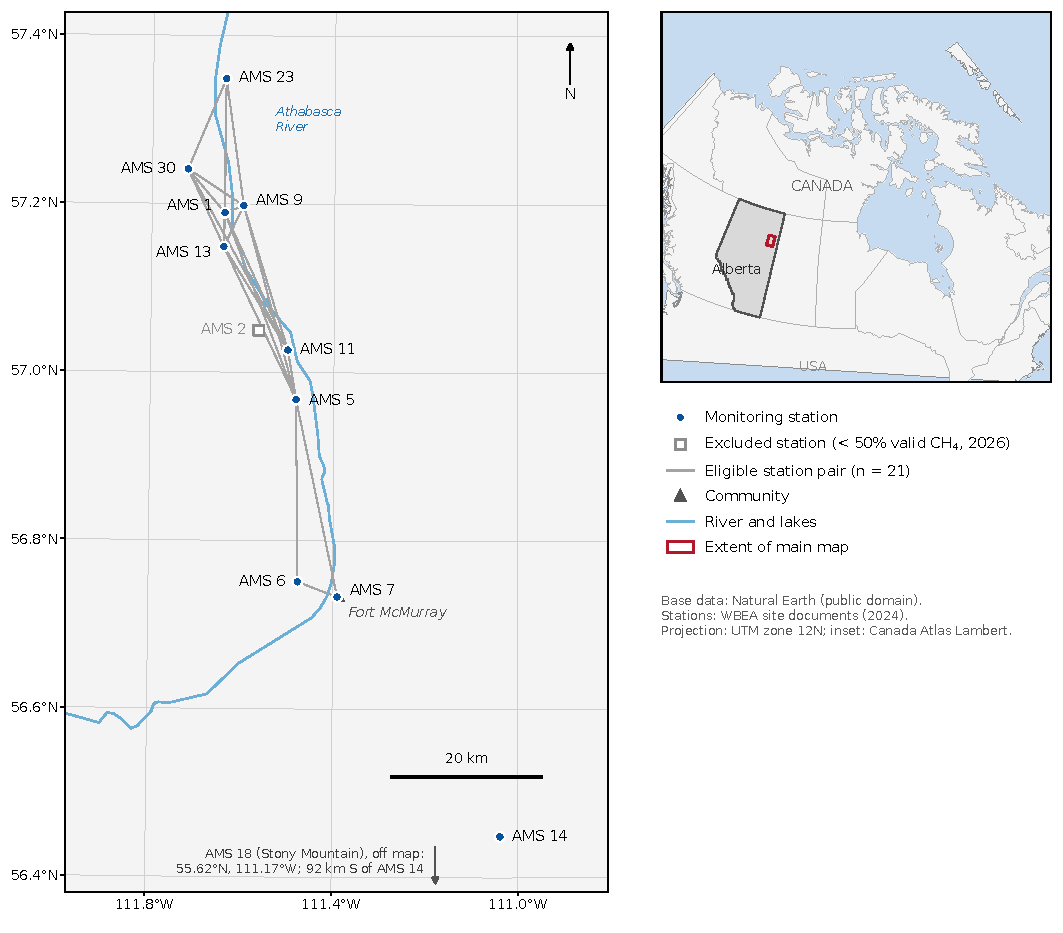
\includegraphics[width=\textwidth]{../figures/section2/fig01_wbea_network.pdf}
\caption{Geographic location and spatial configuration of the Wood Buffalo Environmental Association (WBEA) atmospheric methane monitoring network in northern Alberta, Canada. The maps show the regional location of the study area, the distribution of the 12 monitoring stations, and an enlarged view of the station cluster along the Athabasca River (dashed box). Lines connecting monitoring stations indicate the 21 station pairs eligible for statistical comparison in the 2026 confirmation analysis rather than observed methane transport pathways. The station excluded under the prespecified data-completeness criterion (AMS~2) is shown as an open square. Base data: Natural Earth; station coordinates: WBEA site documents (2024).}\label{fig:network}
\end{figure*}
\begin{table*}[t]
\centering
\caption{Geographic characteristics and meteorological measurement heights of the WBEA atmospheric monitoring stations included in the study.}
\label{tab:stations}
\begin{tabular*}{\textwidth}{@{\extracolsep{\fill}}llrrll@{}}
\toprule
Station & Name & Latitude ($^\circ$N) & Longitude ($^\circ$W) & Wind height (m) & Temperature height (m) \\
\midrule
AMS 1 & Fort McKay - Bertha Ganter & 57.1894 & 111.6406 & 10 & 2, 10 \\
AMS 2 & Mildred Lake & 57.0500 & 111.5641 & 10 & 2 \\
AMS 5 & Mannix & 56.9680 & 111.4821 & 20, 45, 75, 90 & 2, 20, 45, 75, 90 \\
AMS 6 & Patricia McInnes & 56.7514 & 111.4767 & 10 & 2 \\
AMS 7 & Athabasca Valley & 56.7334 & 111.3905 & 10 & 2 \\
AMS 9 & Barge Landing & 57.1982 & 111.5995 & 10, 20 & 2 \\
AMS 11 & Lower Camp & 57.0268 & 111.5008 & 10 & 2 \\
AMS 13 & Fort McKay South & 57.1492 & 111.6423 & 10 & 2 \\
AMS 14 & Anzac & 56.4489 & 111.0380 & 20 & 2 \\
AMS 18 & Stony Mountain & 55.6215 & 111.1728 & 10, 20 & 2 \\
AMS 23 & Fort Hills & 57.3489 & 111.6397 & 10 & 2 \\
AMS 30 & Ells River & 57.2412 & 111.7221 & 10 & 2 \\
\bottomrule
\end{tabular*}
\par\smallskip\begin{minipage}{\textwidth}\footnotesize
Coordinates (WGS84) from WBEA 2024 site documents. Heights (m above ground) list variables with at least 5\% valid hourly values in the 2021--2025 exports; where 10 and 20~m are both listed, the 10~m sensor is used when valid. Methane, total hydrocarbons and non-methane hydrocarbons are reported together at every station (ppm, hourly) by WBEA's continuous hydrocarbon analysers, with an automated zero/span check that occupies one hour per day and is flagged in the data (WBEA SOP-ANA-008; WBEA monthly reports). The analyser model is documented here only for AMS~5 (Thermo~55i, installed 2021); WBEA reports analyser replacements at AMS~5 and AMS~23 in September 2024. AMS~5 has a meteorological tower with sensors at 20--90~m; its 90 minus 20~m temperature difference is the stability measure.
\end{minipage}
\end{table*}

\lipsum[5-6]
\subsection{Datasets and temporal design}
Datasets and temporal partitions are summarised in Table~\ref{tab:data}; observation availability is shown in Fig.~\ref{fig:avail}.
\begin{table*}[t]
\centering
\caption{Observational datasets and temporal design of the methane-monitoring analysis.}
\label{tab:data}
\begin{tabularx}{\textwidth}{@{}l>{\raggedright\arraybackslash}X>{\raggedright\arraybackslash}Xll@{}}
\toprule
Dataset & Variables (units) & Source & Resolution & Years \\
\midrule
Methane & CH$_4$ (ppm) & WBEA continuous monitoring, final validated data & 1~h & 2021--2026 \\
Surface wind & Speed (m\,s$^{-1}$) and direction ($^\circ$) & WBEA continuous monitoring & 1~h & 2021--2026 \\
Air temperature & Temperature ($^\circ$C) at 2--90~m; AMS~5 tower gradient & WBEA continuous monitoring & 1~h & 2021--2026 \\
Boundary-layer height & ERA5 boundary-layer height (m) & Copernicus Climate Change Service, ERA5 & 1~h & 2021--2026 \\
Station locations & Latitude, longitude (WGS84) & WBEA site documents (2024) & -- & -- \\
\bottomrule
\end{tabularx}
\par\medskip
\begin{tabularx}{\textwidth}{@{}ll>{\raggedright\arraybackslash}X@{}}
\toprule
Temporal partition & Dates (MST, hour-ending) & Use \\
\midrule
Development & 1 Jan 2021 01:00 -- 2 Dec 2025 00:00 & Exploratory analysis and method development \\
Reference & 1 Jan 2021 -- 31 Dec 2023 & Fixed station medians, thresholds and stability scaling \\
Confirmation & 1 Jan 2026 01:00 -- 1 Oct 2026 00:00 & Independent confirmation (sealed until methods were frozen) \\
\bottomrule
\end{tabularx}
\par\smallskip\begin{minipage}{\textwidth}\footnotesize
All timestamps are Mountain Standard Time (UTC$-$7, no daylight saving) and refer to the end of the hourly averaging period, as in WBEA reporting. Missing-value handling, station and pair eligibility, and comparison windows are described in Section~3.
\end{minipage}
\end{table*}

\begin{figure*}[!t]
\centering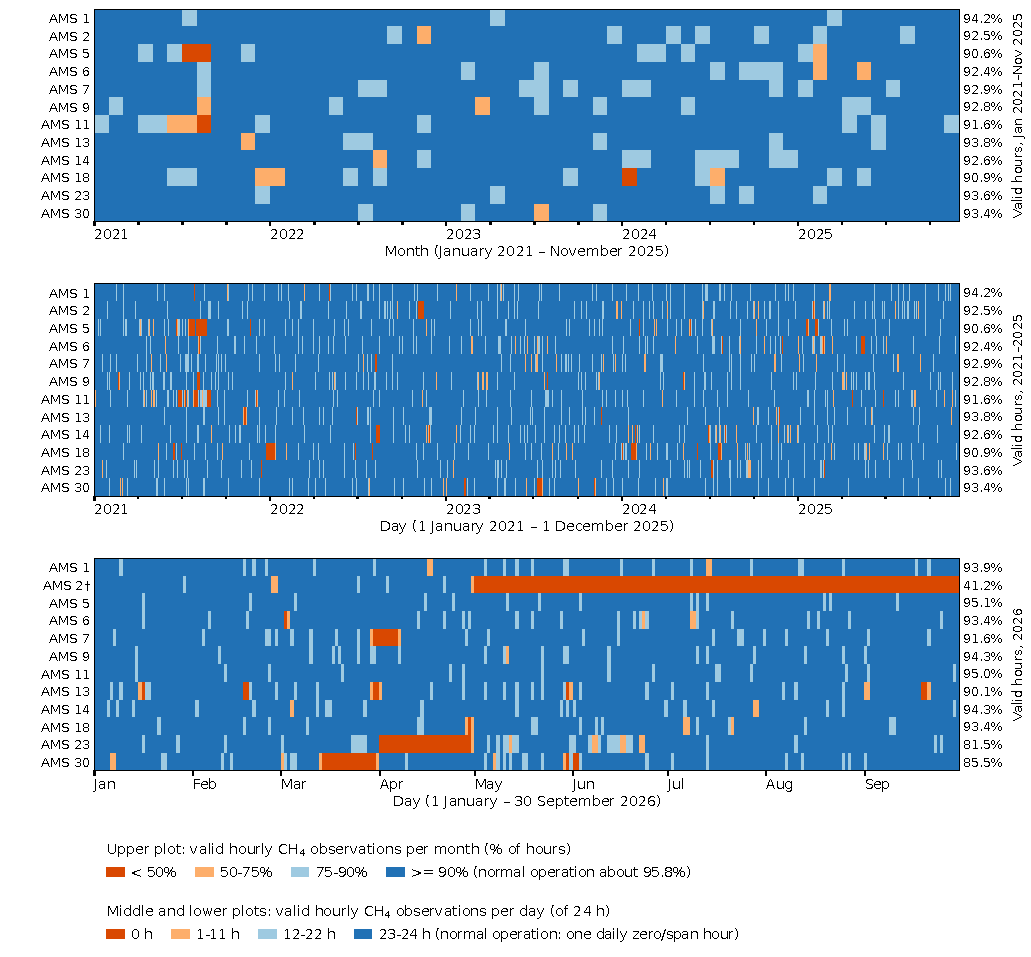
\includegraphics[width=\textwidth]{../figures/section2/fig02_ch4_availability.pdf}
\caption{Availability of hourly methane (CH$_4$) observations at the 12 WBEA monitoring stations. Upper plot: monthly completeness, January 2021 -- November 2025 (development period). Middle plot: daily completeness over the same period. Lower plot: daily completeness, 1 January -- 30 September 2026 (confirmation period). In all three plots completeness is the percentage of hours in the month or day with a valid CH$_4$ value; hours flagged for zero/span checks, calibration, maintenance or invalidity count as missing, and no values are interpolated. Under normal operation one hour per day is used for the automated zero/span check (23 of 24 hours valid; marked on the colour bar). Values at right give each station's share of valid hours in the period. Times are Mountain Standard Time, hour-ending. $^\dagger$AMS~2 was excluded from the 2026 confirmation analysis (41.2\% valid hours).}\label{fig:avail}
\end{figure*}
\lipsum[7-9]

\section{Methods}
\lipsum[10-16]

\clearpage
\begin{thebibliography}{9}
\bibitem[Grange and Carslaw(2019)]{Grange2019} Grange, S.K., Carslaw, D.C., 2019. Using meteorological normalisation to detect interventions in air quality time series. Science of the Total Environment 653, 578--588.
\bibitem[Saha et al.(2025)]{Saha2025} Saha, S., et al., 2025. Dispersion based recurrent neural network model for methane monitoring in Albertan tailings ponds. Journal of Environmental Management 395, 127748.
\bibitem[Uria-Tellaetxe and Carslaw(2014)]{Uria2014} Uria-Tellaetxe, I., Carslaw, D.C., 2014. Conditional bivariate probability function for source identification. Environmental Modelling \& Software 59, 1--9.
\bibitem[Xu et al.(2026)]{Xu2026} Xu, et al., 2026. Physics-informed spatiotemporal analysis of methane concentrations in an oil sands region. Journal of Environmental Management 405, 129618.
\end{thebibliography}
\label{refs:start}
\end{document}
